\section{Processes of the Central Dogma}
Up to this point, we have considered a variety of transport and biosynthetic
processes that are critical to acquiring and generating new cell mass. While
there are of course many other metabolic processes we could consider and
perform estimates of, we now turn our focus to some of the most central processes
which \textit{must} be undertaken irrespective of the growth conditions --
the processes of the central dogma.


\subsection{DNA Replication}
Most bacteria (including \textit{E. coli}) harbor a single, circular chromosome
and can have extra-chromosomal plasmids up to $\sim$ 100 kbp in length. We will focus
our quantitative thinking solely on the chromosome of \textit{E. coli} which
harbors $\approx$ 5000 genes and $\approx 5\times 10^6$ base pairs. To
successfully divide and produce viable progeny, this chromosome must be
faithfully replicated and segregated into each nascent cell. We again rely on
the near century of literature in molecular biology to provide some insight on
the rates and mechanics of this replicative feat, as well as the production of the
required starting materials dNTPs (\FIGSUPP[DNA_synthesis]{dntp}, and discussed in Appendix \nameref{sec:SI_central_dogma}).


Replication is initiated at a
single region of the chromosome termed the \textit{oriC} locus at which a pair
of DNA polymerases bind and begin their high-fidelity replication of the genome
in opposite directions. Assuming equivalence between the two replication forks,
this means that the two DNA polymerase complexes (termed replisomes) meet at the
midway point of the circular chromosome termed the \textit{ter} locus. The
kinetics of the five types of DNA polymerases (I -- V) have been intensely
studied, revealing that DNA polymerase III performs the high fidelity processive
replication of the genome with the other "accessory" polymerases playing
auxiliary roles \citep{fijalkowska2012}. \textit{In vitro} measurements have
shown that DNA Polymerase III copies DNA at a rate of $\approx 600$ nucleotides
per second (BNID: 104120). Therefore, to replicate a single
chromosome, two replisomes (containing two DNA polymerase III each) moving at their maximal rate would copy the
entire genome in $\approx$ 4000 s. Thus, with a division time of 5000 s (our
"typical" growth rate for the purposes of this work), there is sufficient time
for a pair of replisomes complexes to replicate the entire genome.
However, this estimate implies that 4000 s would be the upper-limit time scale
for bacterial division which is at odds with the familiar 20 minute (1200 s)
doubling time of \textit{E. coli} in rich medium.

\begin{figure}
  \centering{
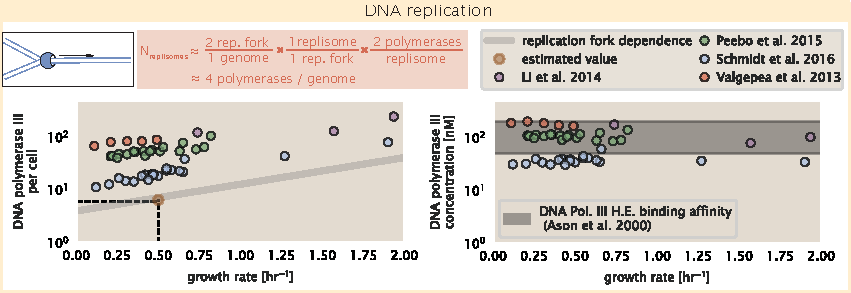
\includegraphics{main_figs/DNA_replication_main.pdf}
\caption{\textbf{Complex abundance estimates for dNTP synthesis and DNA
replication.} An estimate
for the minimum number of DNA polymerase holoenzyme complexes needed to
facilitate replication of a single genome. Points in the left-hand plot correspond
to the total number of DNA polymerase III holoenzyme complexes
([DnaE]$_3$[DnaQ]$_3$[HolE]$_3$[DnaX]$_5$[HolB][HolA][DnaN]$_4$[HolC]$_4$[HolD]$_4$)
per cell. Right-hand plot shows the effective concentration of DNA polymerase III
holoenzyme (See Appendix \nameref{sec:protein_size_SV} for calculate of cell
volumes). Grey lines in left-hand panel show the estimated number of
complexes needed as a function of growth, the details of which are described
in the Supplemental Information.} \label{fig:DNA_synthesis}

\figsupp[Estimate and observations of the abundance of ribonucleotide
reductase, a key component in dNTP synthesis.]{Estimate of the number of
ribonucleotide reductase enzymes needed to facilitate the synthesis of
$\approx 10^7$ dNTPs over the course of a 5000 second generation time. Points
in the plot correspond to the total number of ribonucleotide reductase I
([NrdA]$_2$[NrdB]$_2$) and ribonucleotide reductase II ([NrdE]$_2$[NrdF]$_2$)
complexes. Grey lines in top panel show the estimated number of complexes
needed as a function of growth, the details of which are described in the
Appendix.}{\includegraphics{main_figs/dntp_synthesis.pdf}}\label{figsupp:dntp}
  }
\end{figure}


Even in rapidly growing cultures, where bacteria like \textit{E. coli}
parallelize its DNA replication  with as many as 10 - 12 replication forks at a
given time \citep{bremer2008, si2017},  we expect only a few polymerases
($\approx 10$) are needed. However, as shown in \FIG{DNA_synthesis} DNA
polymerase III is nearly an order of magnitude more abundant. This discrepancy
can be understood by considering its binding constant to DNA. DNA polymerase III
is highly processive, facilitated by a strong affinity of the complex to the
DNA. \textit{In vitro} biochemical characterization has quantified the $K_D$ of
DNA polymerase III holoenzyme to single-stranded and double-stranded DNA to be
50 and 200 nM, respectively \citep{ason2000}. The right-hand plot in
\FIG{DNA_synthesis} shows that the concentration of the DNA polymerase III
across all data sets and growth conditions is within this range. Thus, while the
copy number of the DNA polymerase III is in excess of the strict number required
to replicate the genome, its copy number appears to vary such that its
concentration is approximately equal to the dissociation constant to the DNA.
While the processes regulating the initiation of DNA replication are complex and
involve more than just the holoenzyme, these data indicate that the kinetics of
replication rather than the explicit copy number of the DNA polymerase III
holoenzyme is the more relevant feature of DNA replication to consider. In light
of this, the data in \FIG{DNA_synthesis} suggests that for bacteria like
\textit{E. coli}, DNA replication does not represent a rate-limiting step in
cell division. However, it is worth noting that for bacterium like \textit{C.
crescentus} whose chromosomal replication is initiated only once per cell cycle
\citep{jensen2001}, the time to double their chromosome indeed represents an
upper limit to their growth rate.
